\chapter{Grundlagen}
In diesem Kapitel wird eine Einführung in die Grundlegenden Eigenschaften der untersuchten Systeme gegeben.
Zunächst geht es um die Oberflächen von Festkörpern, da dies in der vorliegenden Arbeit genauer untersucht werden.
Anschließend geht es um den Antiferromagnetismus, welcher die magnetischen Strukturen innerhalb der Proben beschreibt.
Dann geht es um die Wechselwirkung zwischen Oberflächen und Molekühle und wie diese sich auf der Oberfläche bezüglich ihrer geometrischen und elektronischen Struktur verändern.
Zuletzt werden dann die Oberflächen und Molekühle eingeführt, welche zur Präperation der verwendeten Proben genutzt wurden.

    \section{Einkristalloberflächen}
        Die geordneten Strukturen eines Einkristalls kommen durch die Wechselwirkung der Elektronen zwischen den einzelnen Atomen.
        So ergibt sich eine periodische Anordnung der Atome im thermischen Gleichgewicht.
        Dabei sind die Atome nicht komplett starr an ihre Plätze gebunden, sondern führen kleine Schwingungen um diesen aus.
        Mit der Temperatur sinkt auch die Auslenkung.
        Dieses Wechselspiel der strukturellen Ordnung findet sich auch in der elektronischen Struktur wieder.
                
        Wird ein Einkristall entlang einer Kristalleben durchschnitten so ergibt sich eine Oberfläche.
        Die Ebene erhält den Namen der Indizes des auf ihr senkrecht stehenden Gittervektors $r_{hkl}$, also $(hkl)$.
        Als Oberfläche werden die oberen Atomlagen definiert, die sich in der geometrischen und/oder chemischen Art von der des Volumens unterscheiden~\cite{Fauster}.
        Aufgrund der nun fehlenden Bindungen nach oben ergeben sich neue elektronische und geometrische Eigenschaften.
        So kann es zu lateralen und transversalen Verschiebungen gegenüber der volumenartigen Struktur, so genannte Rekonstruktionen und Relaxation kommen.
        Dabei ordnen sich die Atome um, um damit einen energetisch günstigeren Zustand zu erhalten.
    
        Wie im Volumenkristall kann die Oberfläche durch eins von fünf Bravais-Gittern beschrieben werden, wobei auf jedem Gitterpunkt eine atomare Basis gesetzt wird.
        Die Punkte dieses zweidimesionalen Gitters lassen sich durch den Gittervektor
        \begin{equation}
            \vec{r}_{nm} = n \vec{a}_1 + m \vec{a}_2
            \label{eqn:Gittervek}
        \end{equation}
        mit $n,m \in \mathbb{Z}$ und den Vektoren der Einheitszelle $\vec{a}_1, \vec{a}_2$ beschreiben.
        Geimeinsam legt das Bravais-Gitter und die atomare Basis die Symmetrien der Oberfläche fest.
    
        Durch die Anlagerung von Adsorbaten können Symmetrien der Oberfläche verloren gehen.
        Die Struktur der Adsorbate relativ zur Oberfläche wird Überstruktur genannt.
        Durch den meist größeren Abstand der Adsorbate untereinander als der Basen des Substrates ergibt sich auch eine größere Einheitszelle.
        Beim Schneiden der Einkristalle um eine Oberfläche zu erhalten können sich unter anderem auch Stufen ausbilden.
        Vermehrt treten diese Stufen bei hochindizierten Oberflächen auf, wobei einzelne Terrassen dann eine niedrigindizierte Oberfläche darstellen~\cite{Fauster}.
        Diese Stufen oder auch Defekte in der Oberfläche bilden Keimzellen für Anlagerung von Adsorbaten.
        Um die Überstruktur des Adsorbate zu beschreiben wird die von ihnen aufgespannte Einheitszelle aus den Gittervektoren des Substrats rekosntruiert.
        Die Gittervektoren des Übergitters $\vec{b}_1, \vec{b}_2$ lassen sich dann als Matrixschreibweise darstellen.
        Damit ergibt sich auch die Überstrukturmatrix $C$ mit 
        \begin{equation}
            \begin{pmatrix}
                \vec{b}_1 \\
                \vec{b}_2 \\
            \end{pmatrix}
            = 
            \begin{pmatrix}
                C_{11} & C_{12} \\
                C_{21} & C_{22} \\
            \end{pmatrix}
            \begin{pmatrix}
                \vec{a}_1 \\
                \vec{a}_2 \\
            \end{pmatrix}.
        \end{equation}
        Relative Verschiebungen zum Substrat bleiben dabei ohne Beachtung, es zeigt nur die Periodizität der Struktur an.
        Ferner kann es zur Aubildung verschiedener Domänen kommen, besonders dann, wenn die Symmetrie des Übergitters kleiner als die des Substrates ist~\cite{Fauster}.
        Einzelne Domänen weisen Symmetrie äquivalente Anordnungen auf, häufug handelt es sich nur umgedrehte Einheitszellen.
        Nicht nur Adsorbatebedeckungen lassen sich durch diese Notation beschreiben, auch die Rekonstruktion der Oberfläche.
        Hierbei sind es keine Adsorbatatome, sondern die Oberflächenatome selbst, die eine neue Struktur ausbilden.
        Die Relaxation, welche die Änderung im Lagenabstand beschreibt kann hingegen nicht durch dies Notation beschrieben werden.
        Sie ist ebenso wie die Rekonstruktion vom Material, der Kristallstruktur und der Oberflächenorientierung abhängig.
        Einige Rekonstruktionen und Relaxation hängen auch vom Präperationsprozess ab, wenn die Oberfläche selbst metastabil ist.
    
        Wie bereits erwähnt hängen geometrische und elektronische Struktur stark zusammen.
        Sodass sich an Oberflächen durch die fehlenden Bindungen die elektronische Struktur verändern kann.
        Die quantenmechanische Beschreibung der Elektronen erlaubt es auch die elektronischen Zustände der Oberfläche durch Quantenzahlen auszudrücken.
        Hier ist $\vec{k}_{||}$ der Wellenzahlvektor der Oberfläche die Ausschlag gebende Größe um die Oberflächenbandstruktur $E(\vec{k}_{||})$ zu beschreiben.
        Ganz besondere Beachtung erhalten die Zustände nahe der Fermikante $E_\text{F}$ die für leitenden Eigenschaften verantwortlich sind.
        Erhaltene Oberflächenbandstruktur kann von der der Volumenbandstruktur abweichen.
        Dies führt zum Teil zu Oberflächenzuständen, die unterscheiden sich energetisch von denen im Volumenkristall und können somit nur in dessen Bandlücke auftreten.
    
        % Ein wichtiger Ansatz für die periodische Struktur der Oberfläche und dessen elektronischen Zustände ist das Bloch Theorem.
        % Die Oberfläche entspricht einer Anordung äquivalenter Punkte welche durch den Gittervektor aus \autoref{eqn:Gittervek} ineinander überführt werden können

    \section{Antiferromagneten}
        Antiferromagneten (AFM) Zeichen sich dadurch aus, dass Sie nach außen hin kein permanetes magnetisches Moment aufweisen.
        Vereinfacht sind im Inneren die magnetischen Momente vom gleichen Betrag und nebeneinander liegende Momente sind antiparallel unterinander ausgerichtet \cite{Suter}.
        Dieser Zustand ist allerdings nur unterhalb der Néel-Temperatur $T_\text{N}$ stabil, oberhalb verhälten sich die Antiferromagneten paramagnetisch.
        Um das Phänomen des Antiferromagnetismus zu erklären bedarf der quantenmechanischen Erklärung unter Beachtung des Pauli Verbots und der Hundschen Regeln \cite{TUChemnitz}.
        Es ergibt sich der Austauschwechselwirkungshamiltonien $H_\text{A} = - J_{ik} \vec{S_i}\cdot\vec{S_k}$ der die direkte Wechselwirkung der Spins berücksichtigt.
        Für $J_{ik} < 0$ ergibt sich die antiferromagnetische Kopplung und für $J_{ik} > 0$ eine ferromagnetische Kopplung.
        $J_{ik}$ spiegelt dabei die Stärke der Austauschwechselwirkung wieder und folgt aus dem Überlapp der Wellenfunktionen der beteiligten Elektronen.
        Um eine Aussage über die Ordnung im Antiferromagnet zutreffen gibt es den Ordnungsparameter $L = S^{\uparrow} - S^{\downarrow}$.
        Hierbei ist $S^{\uparrow}$ beziehungsweise $S^{\downarrow}$ der Spin der Untergitter.

        \begin{itemize}
            \item fcc Gitter (111) und (100) Oberfläche
            \item real und reziproker Raum
            \item Bandstruktur
            \item Oberflächenzustände?
        \end{itemize}

        % \subsection{Superaustausch}
        % \label{sec:Super}
        \begin{figure}
            \centering
            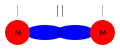
\includegraphics[width=0.6\textwidth]{./content/pictures/AFM2.pdf}
            \caption{Darstellung zur Veranschaulichung der antiferromagnetischen Kopplung.
            Als Ligand fungiert hier ein Sauerstoffatom mit seinem p-Orbital (blau).
            Die Spins der d-Orbitale der Metalle (rot) koppeln ferromagnetische mit denen des Sauerstoffs.
            So entsteht die antiferromagnetische Kopplung der beiden Metallatome.}
            \label{fig:AFM}
        \end{figure}
        Ursache des Antiferromagnetismus ist der Superaustausch.
        Beim Superaustausch koppeln zwei Atome mit einem magnetischen Moment über ein weiteres nicht magnetische Atom. 
        Dabei kann die Kopplung ferro- oder antiferromagnetisch sein, meist jedoch antiferromagnetisch \cite{AFM_1}.
        Sind die beiden koppelnden magnetischen Momente nicht gleich groß, so tritt Ferrimagnetismus auf, es gibt dann eine makroskopische Magnetisierung.
        Der Superaustausch ist winkelabhängig, da es dabei um den Überlapp der Orbitale geht.
        Für die Erklärung wird sich hier nur auf die \SI{180}{\degree} Wechselwirkung beschränkt.
        Beispielhaft ist die Kopplung in \autoref{fig:AFM} dargestellt.
        Es kommt bei diesem indirekten Austausch nicht zu einem Überlapp der spintragenden Wellenfunktionen sondern zu der Vermittlung der langreichweitigen Ordnung über einen Liganden.
        Direkter Austausch sorgt für ferromagnetische Kopplung benachbarter andersartige (nicht magnetische) Atome.
        Zwischen Metall und Ligand herscht also direkte Austauschwechselwirkung und damit eine indirekte Austauschwechselwirkung, der Superaustausch zum übernächsten Atom, einem weiteren Metallatom.
        Bei den vorliegenden Metalloxiden ist es so, dass die Elektronen der Metallatom des nicht vollen 3d Oribtals über die 2p Orbitale des Sauerstoffs koppeln.
        Da dieses Orbital voll ist, müssen die Elektronen unterschiedliche Spinrichtung haben.
        Damit besitzten die Sauerstoffatome auch kein eigenes magnetisches Moment.
        Somit ist dann die Wechselwirkung über das Sauerstoffatom hinweg dann antiferromagnetisch.
        Es ergeben sich so zwei Untergitter, welche unterschiedlicher Spinrichtung sind, die Gesamtmagnetisierung ist also wie für Antiferromagneten erwartet Null.
        % Die Wellenfunktionen der Kationen überlappen nur gering und da die Austauschwechselwirkung nur geringe Reichweiten hat können nur die 3d und 2p überlappen.
        % \begin{itemize}
        %     \item Magnonen
        % \end{itemize}    
            
    
    \section{Wechselwirkung von Oberfläche mit Molekülen}
        Moleküle haben im Gegensatz zu Festkörpern, energetisch separierte Zustände, die Orbitale.
        Werden Molekül auf eine Oberfläche aufgebracht so kommt es zur Wechselwirkung zwischen diesen und der Struktur der Oberfläche.
        Bei der Wechselwirkung von Molekülen mit Oberflächen wird in zwei Arten der Adsorption unterschieden. 
        Zum Einen der Physisorption und der Chemisorption, welche wiederum in stark und schwach unterschieden wird.
        Zwischen den beiden Adsorptionsarten lässt sich durch ihre Bindungsstärke von den Molekülen auf dem Substrat unterscheiden.
        Dabei wird als Bindungsstärke die Energie bezeichnet, die nötig ist um ein Molekül von der Oberfläche zu lösen.
        In beiden Fällen handelt es sich um eine Adsorption die auch die Oberflächenstruktur des Substrates beeinflussen können.
        So können neue Zustände entstehen und vorhandene Eigenschaften stark verändert werden.
        %~\cite{ma-DJ
        
        \subsection{Physisorption}
            Bei der Physisorption spielt maßgeblich die Van-der-Waals-Kraft eine Rolle, hat also eine eher geringe Bindungsenergie der Moleküle zum Substrat~\cite{cinchetti_activating_2017}.
            Charakteristisch für die Physisorption ist die Abwesenheit von chemischen Bindungen sowie einen Substrat-Adsorbat-Abstand von mehr als \SI{3}{\angstrom}. %~\cite{bergenti_spinterface_2019}
            Da die Wechselwirkung bei der Physisorption nur gering ist werden die Eigenschaften der Oberfläche und des Moleküles nur schwach beeinflusst~\cite{bergenti_spinterface_2019}.
            Allerdings kann es beim Substrat zu Relaxation kommen.
            Die Bindungen des Moleküls werden nur schwach beeinflusst, sodass sie den Eigenschaften aus der Gasphase stark ähneln~\cite{cinchetti_activating_2017}.
            Die Van-der-Waals-Kraft gehört zu den elektrostatischen Kräften, es werden also keine Elektronen mit dem Substrat ausgetauscht~\cite{bergenti_spinterface_2019}.
            Allein die Induzierung und Fluktuation von Dipolen führt zu dieser Bindung zwischen Molekül und Substrat.
            Die Van-der-Waals-Kraft kann man in drei Arten unterteilen:
            \begin{itemize}
                \item \textbf{Dipol-Dipol-Kraft:} Sie ist die Kraft zwischen zwei permanenten Dipolen, die Keeson-Wechselwirkung.
                \item \textbf{Dipol-induzierter-Dipol-Kraft:} Die Wechselwirkung zwischen einem induziertem Dipol und einem Dipol wird auch als Debye-Wechselwirkung bezeichnet.
                \item \textbf{Londonsche Dispersions-Wechselwirkung:} Zwischen zwei induzierten Dipolen wirkt die Londonsche Dispersions-Wechselwirkung, sie dominiert meist die Van-der-Waals Kraft.
            \end{itemize}

            Die Physisorption kann durch zwei Potetiale beschrieben werden.
            Das eine Potential wirkt repulsiv und resultiert aus dem Pauliverbot.
            Kommen sich Molekülorbital und Substratorbital zunah, überlappen diese.
            Auf Grund des Pauliverbots dürfen keine zwei Elektronen dann in allen Quantenzahlen übereinstimmen und es resultiert in eine abstoßende Kraft.
            Attraktives Potentential resultiert dabei aus der Debye-Wechselwirkung.
            So kommt es beim Gleichgewicht zu einem stabilen Substrat-Molekül-Abstand.
            Das gesamtpotential ist auch als Lennard-Jones-Potential bekannt.
            Vermehrt tritt die Physisorption bei Halbleitern und Isolatoren auf, da die Molekülzustände in der Bandlücke liegen und so keine Bindung mit dem Substrat eigegangen werden kann~\cite{IF_1}.
        
        \subsection{Chemisorption}
            % Im Gegensatz zur Physisorption findet bei der Chemisorption  ein Austausch von Elektronen stattfinden.
            Im Gegensatz zur Physisorption sind die Bindungen um Einiges stärker und führen somit zu Veränderung am Substrat wie auch den Molekülen~\cite{bergenti_spinterface_2019}.
            Ferner wird von Chemisorption gesprochen, wenn die Stärke der Wechselwirkung größer als \SI{1}{\electronvolt} ist~\cite{muscat_chemisorption_1978}.
            Aber dies allein ist nicht ausschlaggebend, es muss eine chemische Veränderung auftreten.
            Dabei kann es sich um kovalente und ionische Bindungen handeln und es kann zum Ladungsaustausch und/oder Hybridisierung kommen~\cite{harutyunyan_hybridisation_2013}.
            Beim Ladungsaustausch kann ein zunächst unbesetztes Orbital unter die Fermikante rutschen und besetzt werden, es kann also neben den strukturellen auch zu elektronischen Veränderungen kommen.
            Im Gegensatz dazu können bei der Hybridisierung mehrer Zustände vom Molekül und/oder Oberfläche durchmischt werden.
            Verbreiterungen, Verschiebungen und auch Aufspaltungen von Molekülzuständen kann die Folge sein~\cite{IF_1}.

            \begin{figure}
                \centering
                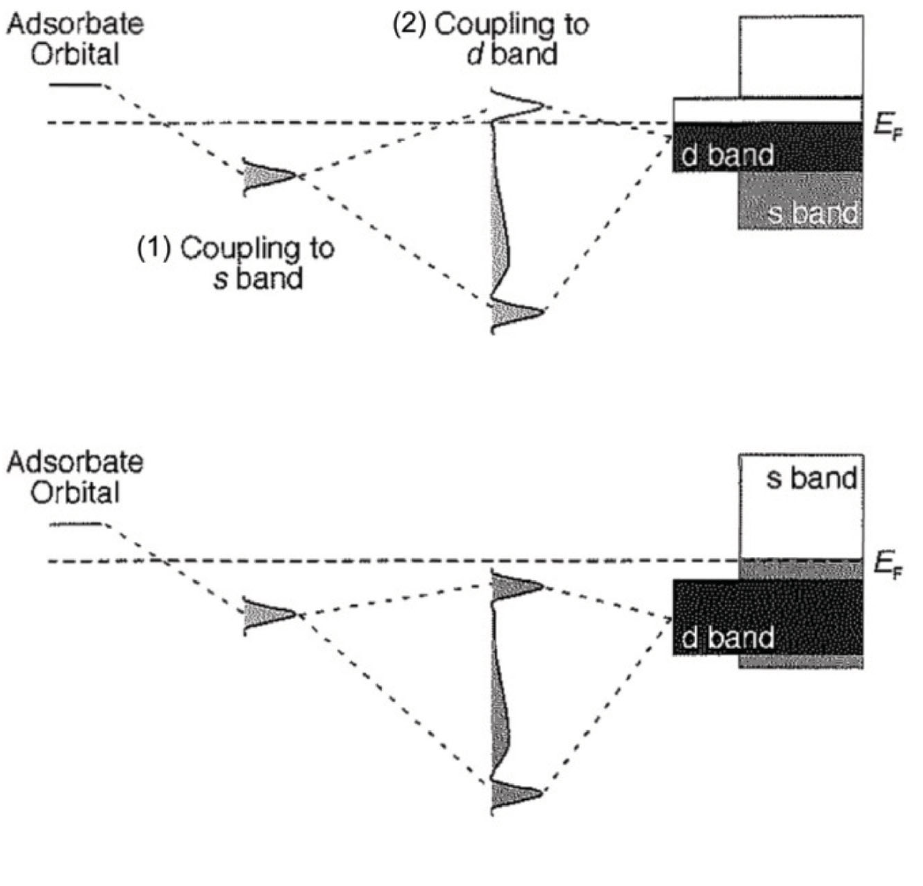
\includegraphics[width=0.6\textwidth]{./content/pictures/Chemisorption2.PNG}
                \caption{Das adsorbierte Molekül hybridiziert mit dem s-/p-Band des Substartes (1), der schwachen Chemisorption.
                In einem weiteren Schritt kommt es dann zur starken Chemisorption durch Einbindung der d-Bänder (2, oben), es entsteht ein bindendes und ein antibindenes Orbital.
                Durch die Lage der d-Bänder werden nun das bindenden und antibindendene Orbital besetzt, dadurch kommt es zu einer repulsiven Kraft und die Bindung wird wieder geschwächt (unten). Aus~\cite{IF_1}.}
                \label{fig:Chemisorption}
            \end{figure}
            Schwache Bindungen werden meist durch die Wechselwirkung mit den breiten s- oder p-Bändern hervorgerufen.
            Wodurch sich das Energieniveau der Moleküle absenkt und verbreitert, siehe dazu in \autoref{fig:Chemisorption}.
            Für die starke Chemisorption folgt ein weiterer Schritt, der nun abgesenkte Zustand überlappt mit dem der näherungsweise d-Bänder.
            Es bilden sich bindende und antibindendene Zustände aus.
            Ja nach Lage des Ferminiveaus wird nur der bindenden Zustand (starke Adsorption) oder auch (nur teilweise) der antibindene Zustand gefüllt, wodurch repulsiv Kräfte auftreten.
            Ferner beeinflusst auch die Ausdehnung der d-Bänder die Stärke der Chemisorption.
        
        \subsection{Selbstanordnung}
            \begin{figure}
                \centering
                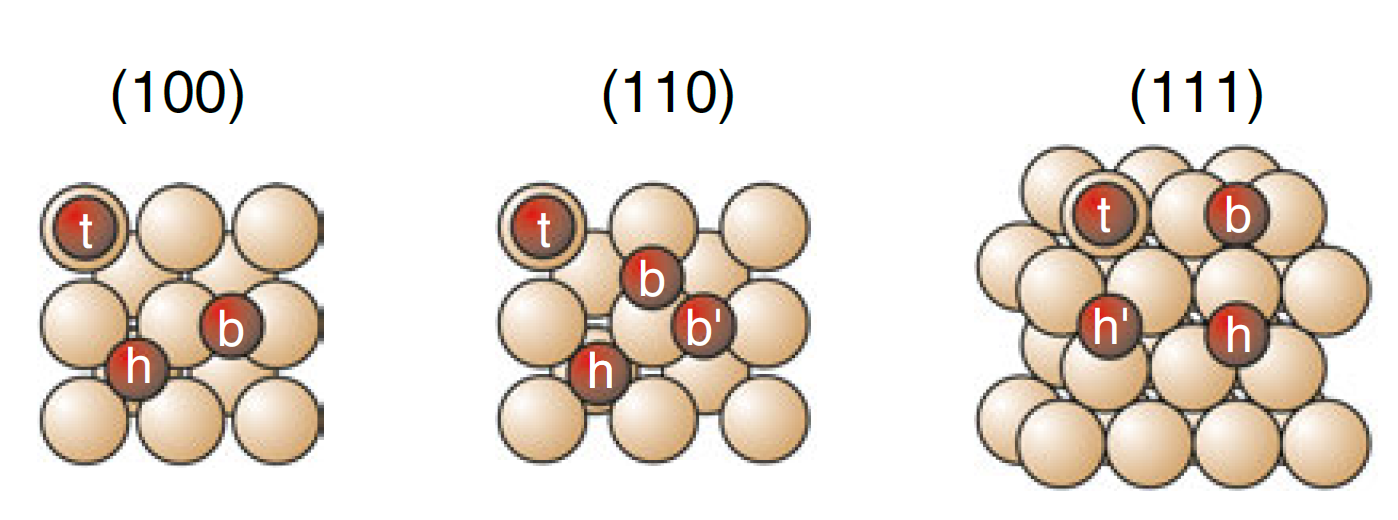
\includegraphics[width=0.6\textwidth]{./content/pictures/Adsorbate}
                \caption{Die Adsorbateplätze für verschieden orientierte Oberflächen eines flächenzentrierten Kristalls.
                Es gibt Plätze direkt oberhalb eines Substratatoms (\textit{on top} - t).
                Zwischen zwei Substratatomen gibt es kurze (b) und lange (b') Brückenplätze (\textit{bridge}), sowie Muldenplätze hexagonaler dicht gepacktester Struktur (\textit{hollow} - h) und flächenzentrierter Struktur (h'). Aus~\cite{Fauster}.}
                \label{fig:Adsorbate}
            \end{figure}
            Einige Moleküle ordnen sich regelmäßig auf dem Substrat an, dieser Effekt wird Selbstanordnung genannt.
            Dabei bilden die Moleküle eine Überstruktur im Vergleich zum Gitter des Substrates.
            Gewünscht ist dies, da dann die Molekül einheitlich auf der Oberfläche orientiert sind und somit auch ihre Orbitale, dies ist notwendig für die Molekülorbital-Tomographie (s. \autoref{sec:MOT}).
            Ferner lassen sich gitteratig verteilte Moleküle gezielter manipulieren, wie es für Anwendungen notwendig ist.
            
            Moleküle stellen eine Art der Adsorbate da und können sich an verschiedene Stellen des Substrates setzen.
            Hier wird auf drei unterschiedeliche Möglichkeiten unterschieden dem Platz direkt über einem Substratatom (\textit{on top}), zwischen zwei Substratatomen (\textit{bridge}) oder in der Mitte von mehreren Substratatomen in einer Mulde (\textit{hollow}).
            Beispielhaft ist dies für einen flächenzentrierten Kristall mit verschiedenen Oberfläche in \autoref{fig:Adsorbate} dargstellt.
            Die physikalische Ursache ist noch nicht ganz klar, warum sich manche Moleküle auf einigen Substraten ordnen und andere hingegen nicht.
            Naheliegend ist, dass es mit der Wechselwirkung zusammenhängt und der Affinität Elektronen auszutauschen.
            Dies wurde bereits auf die Austrittsarbeit für einige Metaloxide hinweg untersucht \cite{greiner_universal_2012}.

            Das Wechselspiel zwischen der Molekül-Molekül-Wechselwirkung und Molekül-Substrat-Wechselwirkung definiert die finale Struktur \cite{IF_1}.
            Dabei sind vor Allem gerichtete Kräfte wichtig um die Regelmäßigkeit zu erhalten.
            Schwächste und ungerichteste Kraft ist die Van-der-Waals-Kraft, genauer die Debye-Wechselwirkung (\SIrange{0.02}{0.1}{\electronvolt}), die allerdings sehr langreichweitig ist.
            Weitere Ursache ist der Einfluss des Substrates auf die Wechselwirkung den Molekülen untereinander, z.B. durch Oszillationen des Oberflächenpotentials.
            Die Keeson-Wechselwirkung als Ursache der Dipol-Dipol-Interaktion hat ebenfalls Beteiligung an der Anordnung der Moleküle, allerdings nur wenn die Moleküle ein permanetes Dipolmoment haben.
            Mit der Wasserstoff-Brücken-Bindung (\SIrange{0.01}{1.73}{\electronvolt}) unter den Molekülen bindet sich ein Wasserstoffatom an ein elektronegativeres Atom, hierdurch kommt es zu Ladungsverschiebung innerhalb der Bindung.
            Das positivere Wasserstoffatom kann nunmehr eine elektrostatische Bindung zu einem weiteren Atom einnehmen.
            Wasserstoff-Brücken-Bindungen sind je stärker sie werden eher geradlinig gerichtete Bindungen mit einer kurzen Bindungslänge.
            Metallisch Koordination ist eine weiter Form der Bindung (\SIrange{0.5}{2}{\electronvolt}), die Moleküle funkieren als Linker zwischen einzelenen Metallatomen.
            Die stärkste und gerichteste Kraft ist jedoch die kovalente Bindung, welche gleichzeitig auch die elektronische Struktur stark beeinflusst.
            Sie ist sogar so stark, dass sie teilweise eine perfekte Selbstanordnung behindert und damit eher zu weniger geordneten Strukturen führen kann \cite{IF_1}.

        \subsection{Energieniveau-Anpassung}
            Für die Anwendung besonders bedeutsam ist die Energieniveau-Anpassung, welche Einfluss auf den Elektronen- und Lochtransport hat~\cite{IF_4}.
            Bei Metalloxiden verschiebt sich durch die Austrittsarbeit die relative Position des Valenz- und Leitungsbandes zum Vakuumniveau \cite{IF_3}.
            Die meisten der Metalloxide haben keine besetzten Zustände nahe der Fermikante, da diese in eine Bandlücke fällt.
            Folglich ist auch Ladungsübertrag vom Substrat auf die Moleküle nur vom Valenz- oder Leitungsband aus möglich.
            Auch wenn einige Oxide Ladungsaustausch zwischen Valenzband und dem höcsten bestzten Molekülorbital (HOMO, \textit{highest occoupied molecular orbital}) zulassen so  gibt es noch kein Model, dass dies beschreibt.
            Verbreitet ist jedoch der Ansatz der Ferminiveau-Anheftung für nicht reaktive Grenzflächen zwischen Molekülen und Oxiden.

            Greiner u.a. \cite{IF_3} fanden heraus, dass die Bandstruktur des Substartes dabei nur eine untergeordnete Rolle spielt.
            Ausschlaggebend für die Energieniveau-Anpassung ist das elektrochemische Potential des Substrates mit dem Reduktionspotentials des Moleküls.
            Genauer die Differenz zwischen der Austrittsarbeit des Substrates und der Ionisationsenergie.
            Als Ionisationsenergie wird die Energie zwischen höchsten besetztem Molekülorbital und dem Vakuumlevel verstanden.
            Die Elektronenaffinität entspricht der Energie zwischen dem Vakuumlevel und dem niedrigsten unbestzten Molekülorbital (LUMO, \textit{lowest unoccoupied molecular orbital}).

            Auch bei Isolatoren kann sich ein Oberflächendipol ausbilden.
            Wegen des Pauliverbot und den zusätzlichen Elektronen der Moleküle an der Grenzfläche werden die Elektronen an der Oberfläche in den Festkörper zurück gedrenkt.
            Durch die Unabhängigkeit vom Adsorptionstyp tritt dieser \textit{Push-Back}-Effekt immer auf~\cite{IF_4} und reduziert damit das Oberflächendipolmoment~\cite{IF_1}.
            Zusätzlich kann das Oberflächendipolmoment durch Ladungsaustausch zwischen Molekül und Substrat geschwächt oder andersherum gestärkt werden.
            Hinzukommend gibt es gegebenfalls noch einen permanenten Dipol des Moleküls, welcher beachtet werden muss.

            \begin{itemize}
                \item charge transfer from HOMO to Ef? \cite{IF_4}
                \item \textbf{Ferminiveau Anheftung}
            \end{itemize}


    \section{Substrate und Molekül Eigenschaften}
        \subsection{Gold (111) Oberfläche}
            Gold gehört zu den Edelmetallen und kristallisiert in der flächenzentrierten Struktur mit einer Gitterkonstanten von \SI{4.08}{\angstrom}~\cite{Marx}.
            Es ist besonders leitfähig, stabil und wenig reaktiv, dennoch rekosntruiert die Oberfläche in einer Fischgräten-Struktur.
            Die Austrittsarbeit der (111)-Oberfläche wurde dabei auf \SI{5.31}{\electronvolt} bestimmt~\cite{Hüfner}.
            Ebenfalls bildet sich auch ein sehr präsenter Oberflächenzustand aus.
            
            Auf Grund der sehr ähnlichen Gitterkonstante zu der des Nickeloxids von nur etwa \SI{2}{\percent} eignet es sich besonders gut als Substrat \cite{NiO_36}.
            \begin{itemize}
                \item Ebenenabstand in Au(111) $d_0 = \SI{2.35}{\angstrom}$.\textbf{\cite{5A_1}}
            \end{itemize} 

        \subsection{Nickeloxid (111) Oberfläche}
            \begin{figure}
                \centering
                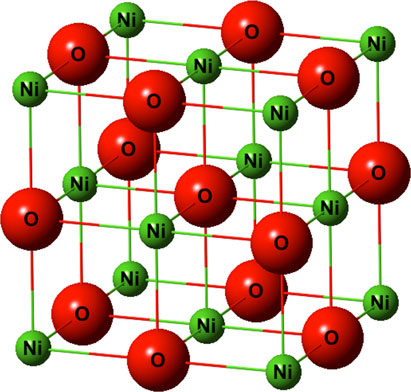
\includegraphics[width=4cm]{./content/pictures/NiO/NiO-structure.jpg}
                \caption{Die Krsiatllstruktur von Nickeloxid. Das $\ce{Ni}^{2+}$ Ion befindet sich in einer oktraedischen Umgebung von $\ce{O}^{2-}$ Ionen. Aus~\cite{NiO-structure}.}
                \label{fig:NiO-structure}
            \end{figure}
            Nickeloxid besitzt die Struktur von \ce{NaCl} und ist in \autoref{fig:NiO-structure} dargestellt~\cite{kunz_chemisorption_1985}. 
            Die geometrische Gitterkonstante beträgt \SI{4.17}{\angstrom}~\cite{sebbari_uranyl_2012}.
            Für die magnetische Ordnung ergibt sich die dopplte Gitterkonstante zwischen zwei gleich ausgerichteten Spins~\cite{Suter}.
            Die Austrittsarbeit lässt sich dabei durch die Präperation beeinflussen und liegt zwischen \SIrange[range-phrase=' und ']{4.5}{5.2}{\electronvolt} \cite{poulain_electronic_2020}.
            % Neutronenbeugung auf Spin empfindlich also dopplte Einheitszelle, anders als die chemisch empfinliche Röntgenbeugung.

            Nickeloxid gehört zu der Familie der Antiferromagneten mit einer Neél-Temperatur von \SI{525}{\kelvin}.
            Da das 3d Band des Nickels im Oxid nur teilweise gefüllt ist (acht von zehn möglichen Elektronen) würde man erwarten, dass es sich hierbei um einen Leiter handelt~\cite{kunz_chemisorption_1985}.
            Dies ist allerdings nicht so und Nickeloxid ist ein Isolator, genauer ein Ladungs-Transferisolator.
            Die thermische Bandlücke liegt bei \SI{3.6}{\electronvolt}~\cite{kunz_chemisorption_1985}.

            Ein Oberflächendipolelement ist besonders stark in der (111)-Orientierung ausgeprägt, da bei der polaren Oberfläche entweder nur Sauerstoff oder nur Nickelionen in der obersten Lage vorhanden sind~\cite{NiO_8}.
            Dies liegt an der Bindung zwischen dem Sauerstoff und dem Nickel.
            Das Oberflächenpotential ist folglich divergent und somit die Oberfläche instabil.
            Problematisch an dünnen Filmen von Nickeloxid in der (111)-Orientierung ist diese Instabilität und die starke Abhänigkeit vom Präperationsprozess \cite{NiO_36}.
            Es gibt verschiedene Beobachtungen zu der Stabilisierung der polaren Oberfläche wie die Rekonstruktion oder \ce{OH-}-Terminierung \cite{NiO_36, NiO_35, NiO_34, NiO_27, NiO_10}.
            Bei der Stabilisierung wird die Oberflächenladung reduziert und damit das Oberflächenpotential gesenkt in Folge dessen es zur Ausbildung einer stabilen Oberfläche kommt.

            Die Magnetisierung ist ebenso wie die Atome abwechseln geschichtet.
            So tritt zunächst eine Ebene mit Nickel auf, in der die Magnetisierung antiparallel zu der nächsten Schicht Nickel ist.
            Denn die Spins innerhalb einer (111)-Ebene koppeln ferromagnetisch wohingegen die Kopplung unter den Ebenen antiferromagnetisch ist~\cite{FeO_6}.

            Nickeloxid zeigt bereits für andere Orientierung für einige Moleküle Chemisorption, was durch enthaltene Defekt hervorgerufen wird~\cite{kunz_chemisorption_1985}.
            Auf Grund dessen eignet sich das Substrat zur Untersuchung bestens, zumal für polare Oberflächen auch eine größere Reaktivität vorhergesagt wird \textbf{Quelle}.
            \begin{itemize}
                \item elektronische Struktur
            \end{itemize}
        \subsection{Eisen (100) Oberfläche}
            \begin{itemize}
                \item WKF
                \item Symmetrie - p4mm
                \item Gitterkonstante ist $a = \SI{2.866}{\angstrom}$
                \item bcc Struktur
            \end{itemize}

        \subsection{Eisenoxid (100) Oberfläche}
            Ebenso wie das Nickeloxid kristallisiert auch das Eisenoxid, welches auch Wüstite genannt wird, in der \ce{NaCl}-Struktur~\cite{FeO_4}.
            Dabei beträgt die Gitterkonstante \SI{3.07}{\angstrom}~\cite{FeO_1} und die $\ce{Fe}^{2+}$-Ionen befinden sich einer oktraedischen Position zum Suaerstoff~\cite{FeO_4}.
            Es handelt sich ebenfalls um einen Isolator mit antiferromagnetischen Eigenschaften und einer Neél-Temperatur von \SI{198}{\kelvin}~\cite{FeO_4}.

            Genau wie in Nickeloxid sind auch hier die (111)-Ebenen untereinander antiferromagnetisch gekoppelt.
            So ergibt sich auf der (100)-Oberfläche abwechselnd Spin ausgerichtete
            nicht-stöchiometrische Verbindung wie das Eisenoxid enthalten dabei verschiedene Oxidationszustände also nicht nur Fe2+ sondern auch \SIrange{10}{32}{\percent} Fe3+ \cite{FeO_11}.
            Fe2+ befinden sich in oktraedischer Umgebung
            O anions and metal cations
            Fe2+ magnetic moments aligned parallel to the close packed (111) planes, but in opposite directions from one plane to the next. The Fe defect clusters discussed above are thought to affect the magnetic properties 

            \begin{itemize}
                \item WKF
                \item Symmetrie - p4mm
            \end{itemize}

        \subsection{Pentacene} \label{sec:5A}         
            \begin{figure}
                \centering
                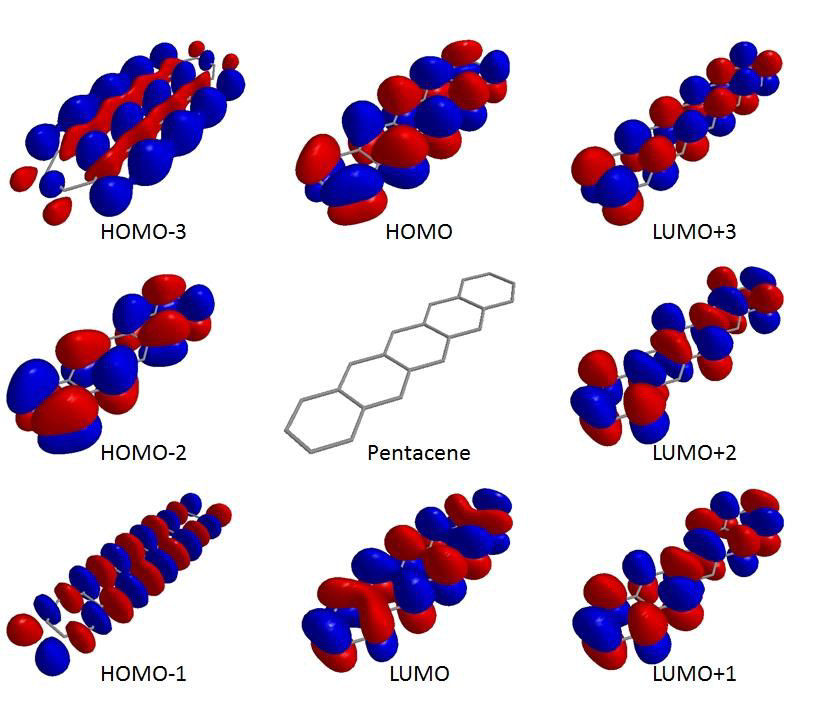
\includegraphics[width=0.6\textwidth]{./content/pictures/PEN.jpg}
                \caption{Geometrische Struktur des Pentacene sowei die vier höchsten besetzten und vier niedrigesten unbesetzen Orbitale. Vorlage aus~\cite{PEN}.}
                \label{fig:PEN}
            \end{figure}
            Bei Pentacene ($\ce{C22H14}$) oder auch kurz 5A handelt es sich um einen Elektronendonator und gehört zu den p-Typ Halbleiter~\cite{5A_1}.
            Seine Struktur ist in \autoref{fig:PEN} dargestellt, welche sich aus linear an Kanten verschmolzenen Phenylringen zusammensetzt~\cite{MM_2}.
            Ebenfalls zu sehen sind jeweils die ersten vier höchsten besetzen und niedrigesten unbesetzten Zustände.
            Die Synthese des Pentacene ist auf Grund der einfachen Struktur ebenfalls einfach.
            Pentacene bringt die perfekten Eigenschaften für Molekülorbitaltomographie mit, da es sich um ein \pi-konjugiertes Molekühl handelt~\cite{MM_2}.

            In dünnen Filmen aus Pentacene zeigt sich eine hohe Elektronenbeweglichkeit.
            Auf der Gold(111)-Oberfläche ordnet es sich an und liegt parallel zum Substrat.
            Der Abstand zwischen den Molekülen und Substrat wird auf \SI{3.28}{\angstrom} bestimmt, was auch in der Größenordnung für Physisorption liegt~\cite{5A_1}.
            

            Dichte von \SI{1.232(6)}{\gram\per\cubic\centi\meter}~\cite{CAS}.
            